\documentclass[12pt,compress,aspectratio=169]{beamer}

\mode<presentation>
{
%  \usetheme{Warsaw}
  \usetheme{Singapore}
%  \setbeamertemplate{navigation symbols}{} % suppress nav bar
%  \setbeamercovered{transparent}
}
\usefonttheme{professionalfonts}
\usepackage{graphicx}
\usepackage{tikz}
\usepackage{amsmath}
\usepackage{mathpazo}
\usepackage[scaled]{helvet}
\usepackage{xcolor,colortbl}
\usepackage{hyperref}
\usepackage{siunitx}

\sisetup{number-math-rm=\mathnormal}

\title{Class 22a: Special Relativity}
\subtitle{Advanced Placement Physics}
\author[TML]{Dr.\ Timothy Leung}
\institute{Olympiads School}
\date{Summer 2018}

\newcommand{\mb}[1]{\mathbf{#1}}
\newcommand{\pic}[2]{\includegraphics[width=#1\textwidth]{#2}}
\newcommand{\bigsqrt}{\ensuremath\sqrt{1-\left(\frac{v}{c}\right)^2}}
\newcommand{\lorentz}{\ensuremath\frac{1}{\bigsqrt}}

\begin{document}

\begin{frame}
  \maketitle
\end{frame}


\begin{frame}
  \frametitle{Introduction}
  The slides on \textbf{special relativity} is a condensed version of the
  slides used for Physics 12 (and with a little bit of calculus). For many of
  you, this will be a review.
\end{frame}


\begin{frame}
  \frametitle{Newtonian (Classical) Relativity}
  \begin{itemize}
  \item In Newtonian physics, space and time are absolute:
    \begin{itemize}
    \item \SI{1}{m} is \SI{1}{m} no matter where you are in the universe
    \item \SI{1}{s} is \SI{1}{s} no matter where you are in the universe
    \item \SI{1}{kg} is \SI{1}{kg} no matter where you are in the universe
    \end{itemize}
  \item Space and time are absolute, therefore velocities are relative:
    \emph{all measured velocities depend on the observer's relative motion}
  \item Our kinematic and dynamic equations applies to all \emph{inertial}
    frames of reference
  \end{itemize}
\end{frame}


\begin{frame}
  \frametitle{Maxwell's Equations in a Vacuum}
  \framesubtitle{Everything Comes Back to This}

  \vspace{-.3in}{\Large
    \begin{align*}
      \nabla\cdot\mb{E} &= 0\\
      \nabla\cdot\mb{B} &= 0\\
      \nabla\times\mb{E} &=-\frac{\partial\mb{B}}{\partial t}\\
      \nabla\times\mb{B} &=\mu_o\varepsilon_o\frac{\partial\mb{E}}{\partial t}
    \end{align*}
  }
  
  \vspace{-.15in}Disturbances in $\mb{E}$ and $\mb{B}$ travel as an
  ``electromagnetic wave'', with a speed:

  \vspace{-.25in}{\Large
    \begin{displaymath}
      c=\frac{1}{\sqrt{\varepsilon_0\mu_0}}=\SI{299792458}{m/s}
    \end{displaymath}
  }
\end{frame}


\begin{frame}
  \frametitle{Peculiar features of Maxwell's equation}
  \begin{itemize}
  \item Makes no mention of the \emph{medium} in which EM waves travels
  \item When applying \emph{Galilean transformation} (classical equation for
    calculating \emph{relative velocity}) to Maxwell's equations:
  \item Gauss's law for magnetism break down: magnetic field lines appear to
    have beginnings/ends
  \item In \emph{some} inertial frames of reference,
    Maxwell's equations are valid and elegant, but in another inertial frame
    of reference, they are ugly
  \item Physicists at the time theorized that---perhaps---there is/are actually
    \emph{preferred} inertial frame(s) of references
  \item This violate the long-standing
    \emph{principle of relativity}, which says that
    \emph{the laws of physics are equal in all inertial frames of reference}
  \end{itemize}
\end{frame}



\begin{frame}
  \frametitle{Making The Equations Work Again}
  Maxwell's equations didn't ``fail''; it was our understanding of space and
  time that needed to change
  \begin{itemize}
  \item Albert Einstein believed in the principle of relativity, and rejected
    the concept of a preferred frame of reference
  \item The speed of an electromagnetic wave (speed of light) must be
    independent of the frame of reference
  \item The failure of the Michelson-Morley experiment which sought to
    experimentally demonstrate the flow of ``ether'' merely
  \item In order to make the equations to work again, Einstein revisited two
    most fundamental concepts in physics: space and time
  \end{itemize}
\end{frame}


\begin{frame}
  \frametitle{Einstein's Postulates on Relativity}
  \begin{block}{The Principle of Relativity}
    All laws of physics must apply equally in all inertial frames of reference.
  \end{block}

  \begin{block}{The Principle of Invariant Light Speed}
    As measured in any inertial frame of reference, light is always propagated
    in empty space with a definite velocity $c$ that is independent of the
    state of motion of the emitting body.
  \end{block}
  
  \vspace{.15in}Published in 1905 in the article
  \emph{On the Electrodynamics of Moving Bodies} when Einstein was 26 years old
  working as a patent clerk in Switzerland
\end{frame}


\begin{frame}
  \frametitle{What's so Special About Special Relativity?}
  \begin{itemize}
  \item\textbf{Classical (Newtonian) relativity:} space and time are
    absolute---speed of light must be relative to the observer
  \item\textbf{Einstein relativity:} speed of light is absolute---space and
    time must be relative to the observer
  \item We must modify our traditional concepts:
    \begin{itemize}
    \item Measurement of space (our coordinate system)
    \item Measurement of time (our clock)
    \item Concept of simultaneity (whether or not two events happens at the
      same time)
    \end{itemize}
  \end{itemize}
\end{frame}



\begin{frame}
  \frametitle{Simultaneity: Thought Experiment}
  Lightning bolt strikes the ends of a moving train
  \begin{center}
    \pic{.58}{87-1-1024x673.png}
  \end{center}
  \vspace{-0.1in}
  \begin{itemize}
  \item The man on the ground sees the lightning bolt striking at the same time
  \item The woman on the moving train sees the lightning bolt on the right first
  \end{itemize}
\end{frame}


\begin{frame}
  \frametitle{Simultaneity}
  \begin{itemize}
  \item Both observers cannot agree on the result, but
    \begin{itemize}
    \item Neither person is wrong
    \item Neither person is misinformed
    \end{itemize}  \item Both are valid inertial frames of reference
  \end{itemize}
  This means that:
  \begin{itemize}
  \item Simultaneity depends on your motion
  \item\textbf{Events that are simultaneous in one inertial frame of reference
    are generally not simultaneous in another.}
  \end{itemize}
\end{frame}

\begin{frame}
  \frametitle{Time Dilation: A Thought Experiment}
  \begin{center}
    \pic{0.4}{light-a-b.png}
  \end{center}
  I'm on a spaceship travelling in deep space, and I shine a light from
  $A$ to $B$. The distance between $A$ and $B$ is really just:

  \vspace{-0.2in}{\LARGE
    \begin{displaymath}
      |AB|=c\Delta t_0
    \end{displaymath}
  }

  \vspace{-0.2in}
  I know the speed of light $c$, and I know how long it took for the light
  pulse to reach $B$. (The reason I used $\Delta t_0$ will be obvious later.)
\end{frame}


\begin{frame}
  \frametitle{Time Dilation: A Thought Experiment}
  \begin{center}
    \pic{.7}{light-a-b-rocket.png}
  \end{center}
  You are in space station watching my spaceship go past you at speed $v$. You
  would see that same beam of light travel from $A$ to $B'$ instead.
  \begin{center}
    \pic{.7}{light-a-b-prime.png}
  \end{center}
\end{frame}

\begin{frame}
  \frametitle{Abandoning Concept of Absolute Time: Time Dilation}
  \framesubtitle{A ``thought experiment''}
  \begin{center}
    \pic{.7}{dilation.png}
  \end{center}
  \begin{align*}
    c^2\Delta t^2 &=v^2\Delta t^2 + c^2\Delta t_0^2\\
    \left(c^2-v^2\right)\Delta t^2 &=c^2\Delta t_0^2\\
    \left(1-\frac{v^2}{c^2}\right)\Delta t^2 &=\Delta t_0^2\\
    \Delta t &=\frac{\Delta t_0}{\bigsqrt}
  \end{align*}
\end{frame}


\begin{frame}
  \frametitle{Time Dilation}
  {\Large
    \begin{displaymath}
      \boxed{\Delta t =\frac{\Delta t_0}{\bigsqrt}}
    \end{displaymath}
  }
  \begin{itemize}
  \item $\Delta t_0$ is called the \textbf{proper time}. It is the time measured
    by a person at rest relative to the object or event.
  \item $\Delta t$ is called the expanded time or \textbf{dilated time}. It is 
    the time measured by a moving observer in another inertial frame of
    reference. Since $\bigsqrt$ is always smaller than 1, $\Delta t$ is always
    greater than $\Delta t_0$.
  \end{itemize}
\end{frame}

\begin{frame}
  \frametitle{Example Problem (A Simple One)}
  \textbf{Example 1a:} A rocket speeds past an asteroid at 0.800$c$. If an
  observer in the rocket sees \SI{10.0}{s} pass on her watch, how long would
  that time interval be as seen by an observer on the asteroid?

  \uncover<2->{
    \vspace{.3in}
    \textbf{Example 1b:} A rocket speeds past an asteroid at 0.800$c$. If an
    observer in the \emph{asteroid} sees \SI{10.0}{s} pass on his watch, how
    long would that time interval be as seen by an observer on the
    \emph{rocket}?
  }

  \uncover<3->{
    \vspace{.3in}
    How can that be?!
  }
\end{frame}


\begin{frame}
  \frametitle{Length Contraction}
  Captain Quick is a comic book hero who can run at nearly the speed of light.
  In his hand, he is carrying a flare with a lit fuse set to explode in
  \SI{1.5}{\micro s}. The flare must be placed into its bracket before this
  happens. The distance ($L$) between the flare and the bracket is \SI{402}{m}.
\end{frame}


\begin{frame}
  \frametitle{Length Contraction}
  \framesubtitle{Another Example}
  \begin{center}
    \pic{.85}{captain-quick.png}
  \end{center}
\end{frame}


\begin{frame}
  \frametitle{Length Contraction}
  If Captain Quick runs at \SI{2.00e8}{m/s}, according to classical mechanics,
  he will not make it in time:
  \begin{displaymath}
    \Delta t= \frac{L}{v}=\frac{\SI{402}{m}}{\SI{2.00e8}{m/s}}
    =\SI{2.01e-6}{s}=\SI{2.01}{\micro s}
  \end{displaymath}
  But according to relativistic mechanics, he makes it just in time\ldots
\end{frame}

\begin{frame}
  \frametitle{Length Contraction}
  To a stationary observer, the time on the flare is slowed:
  \begin{displaymath}
    \Delta t 
    = \frac{\Delta t_0}{\bigsqrt}
    = \frac{\SI{1.5e-6}{s}}{\sqrt{1-\left(\frac{2}{3}\right)^2}}
    = \frac{\SI{1.5e-6}{s}}{0.7454}
    = \SI{2.01e-6}{s}
  \end{displaymath}
  The stationary observer sees a passage of time of
  $\Delta t=\SI{2.01}{\micro s}$, but
  Captain Quick, who is in the same reference frame as the flare, experiences
  a passage of time of $\Delta t_0=\SI{1.50}{\micro s}$, precisely the time for
  the flare to explode.
\end{frame}

\begin{frame}
  \frametitle{Length Contraction}
  \begin{itemize}
  \item So, if Captain Quick sees only $\Delta t_0=\SI{1.50}{\micro s}$, then
    how far did he travel?
  \item He isn't travelling any faster, so he only other possibility is that
    \textbf{the distance actually got shorter} (in his frame of reference).
  \item How much did the distance contract?
  \end{itemize}
  
  \vspace{-.3in}{\LARGE
    \begin{displaymath}
      \boxed{L=L_0\bigsqrt}
    \end{displaymath}
  }

  For this example:
  \begin{displaymath}
    L=L_0\bigsqrt=(\SI{402}{m})\cdot\sqrt{1-\left(\frac{2}{3}\right)^2}
    =\SI{300}{m}
  \end{displaymath}
\end{frame}

  
\begin{frame}
  \frametitle{Lorentz Factor}
  The \textbf{Lorentz factor} $\gamma$ is a short-hand for writing length
  contraction, time dilation and relativistic mass:

  \vspace{-.2in}{\LARGE
    \begin{displaymath}
      \boxed{\gamma=\lorentz}
    \end{displaymath}
  }
  Then time dilation and length contraction can be written simply as:
  {\LARGE
    \begin{displaymath}
      \boxed{\Delta t = \gamma \Delta t_o}\quad\boxed{L = \frac{L_o}{\gamma}}
    \end{displaymath}
  }
\end{frame}



\begin{frame}
  \frametitle{Summary}
  \begin{center}
    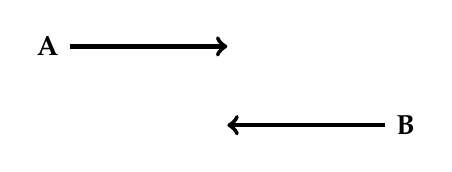
\begin{tikzpicture}[scale=2]
      \draw[ultra thick,->] (1,.5)--(2,.5) node[pos=0,left]{\textbf{A}};
      \draw[ultra thick,->] (3,0)--(2,0) node[pos=0,right] {\textbf{B}};
    \end{tikzpicture}
  \end{center}
  If Person A and Person B are moving at constant speed with respect to one 
  another (doesn't matter if they're moving towards, or away from each other)
  \begin{itemize}
  \item They cannot agree whether any events happens at the same time or not
  \item Each sees the other's clock running slow
  \item Each sees the other ``contracted'' in length along the direction of
    motion
  \end{itemize}
\end{frame}


%\begin{frame}
%  \frametitle{Example Problem}
%  \textbf{Example 2:} A spacecraft passes Earth at a speed of \SI{2.00e8}{m/s}.
%  If observers on Earth measure the length of the spacecraft to be
%  \SI{554}{m}, how long would it be according to its passengers?
%\end{frame}


\begin{frame}
  \frametitle{Relativistic Momentum}
  In Unit 2, you were taught that momentum is mass times velocity. And back in
  Physics 11, you were taught that velocity is displacement over time:

  \vspace{-.2in}{\LARGE
    \begin{displaymath}
      \mb{p}=m\mb{v}=m\frac{d\mb{x}}{dt}
    \end{displaymath}
  }

  \vspace{-.1in}Now that you know both $\mb{x}$ and $t$ depends on the motion,
  we can find the ``relativistic version'' of momentum  for when $\mb{v}$ is
  high compared to $c$):
  
  \vspace{-.35in}{\LARGE
    \begin{displaymath}
      \mb{p}=m_0\frac{d\mb{x}}{dt_0}
      =\frac{m_0d\mb{x}}{\bigsqrt dt}
      =\frac{m_0\mb{v}}{\bigsqrt}
    \end{displaymath}
  }
\end{frame}



\begin{frame}
  \frametitle{Relativistic Mass}
  Based on the momentum equation, we can see that mass is also relativistic:
  {\LARGE
    \begin{displaymath}
      \boxed{m=\frac{m_0}{\bigsqrt}}
    \end{displaymath}
  }
  Mass increases with velocity. At $v=c$, $m=\infty$! But is it \emph{real}?
\end{frame}



\begin{frame}
  \frametitle{Force and Work}
  Knowing the relationship between force and momentum, and the definition of
  work by a force:
  
  \vspace{-.25in}{\LARGE
    \begin{displaymath}
      \mb{F}=\frac{d\mb{p}}{dt}
      \quad\quad
      W=\int\mb{F}\cdot d\mb{x}
    \end{displaymath}
  }

  \vspace{-.1in}Substitute the expression for force into the definition
  of work, then substitute expression for relativistic momentum, and after
  some calculus, we get an expression for kinetic energy:
  
  \vspace{-.3in}{\LARGE
    \begin{displaymath}
      W=\Delta K=\frac{m_0c^2}{\bigsqrt}-m_oc^2
    \end{displaymath}
  }
\end{frame}

\begin{frame}
  \frametitle{Relativistic Energy}
  {\LARGE
    \begin{displaymath}
      \boxed{K=mc^2-m_0c^2}
    \end{displaymath}
  }
  where
  \begin{itemize}
  \item $m_0$ = rest mass = mass as measured in a stationary frame of reference
  \item $m$ = relativistic mass = $m_0/\bigsqrt$
  \item $K$ = kinetic energy
  \item $c$ = speed of light
  \end{itemize}
\end{frame}

\begin{frame}
  \frametitle{Relativistic Energy}
  {\LARGE
    \begin{displaymath}
      \boxed{K=mc^2-m_0c^2}
    \end{displaymath}
  }
  \begin{itemize}
  \item An object of mass $m$ has energy $E_0=m_0c^2$ even when it is not
    moving (this is called \emph{rest energy}
  \item If it \emph{is} moving, then it has a \emph{total} energy of
    $E_T=mc^2$
  \item Kinetic energy $K$ is the difference between total energy and rest
    energy
  \item Whenever there is a change of energy, there is also a change of mass
    \begin{itemize}
    \item ``Conservation of mass'' and ``conservation of energy'' must be
      combined into a single concept of \textbf{conservation of mass-energy}
    \end{itemize}
  \end{itemize}
\end{frame}


\begin{frame}
  \frametitle{Kinetic Energy: Classical vs.\ Relativistic}
  \begin{columns}
    \column{0.5\textwidth}
    \textbf{Relativistic:}
    {\Large
      \begin{displaymath}
        K=\frac{m_0c^2}{\bigsqrt}-m_oc^2
      \end{displaymath}
    }
    \column{0.5\textwidth}
    \textbf{Newtonian:}
    {\Large
      \begin{displaymath}
        K=\frac{1}{2}mv^2
      \end{displaymath}
    }
  \end{columns}
  But are they really different? If we do a series expansion of the
  square-root term, we get:

  \vspace{-.35in}
  {\Large
    \begin{displaymath}
      K =
      m_0c^2
      \left(1+\frac{1}{2}\frac{v^2}{c^2}+\cdots \right) -
      m_0c^2 \approx\frac{1}{2}mv^2+\cdots
    \end{displaymath}
  }
  When $v$ is small compared to $c$
\end{frame}


\begin{frame}
  \frametitle{Comparing Classical and Relativistic Energy}
  \begin{columns}
    \column{0.5\textwidth}
    Classical mechanics:
    {\LARGE
      \begin{displaymath}
        K=\frac{1}{2} mv^2
      \end{displaymath}
    }
    Relativistic mechanics:
    {\LARGE
      \begin{align*}
        K&=mc^2-m_oc^2\\
      \end{align*}
    }
    \column{.5\textwidth}
    \pic{1}{e_k.png}
  \end{columns}
\end{frame}

%\begin{frame}
%  \frametitle{Example Problem}
%  \textbf{Example 4:} A rocket car with a mass of \SI{2.00e3}{kg} is accelerated
%  from rest to \SI{1.00e8}{m/s}. Calculate its kinetic energy:
%  \begin{enumerate}
%  \item Using the classical equation
%  \item Using the relativistic equation
%  \end{enumerate}
%\end{frame}
%
\end{document}
